
\section{Benchmark EP}
\subsection{Wyniki benchmarków - platforma ARM64}
\begin{figure}[H]
    \centering
    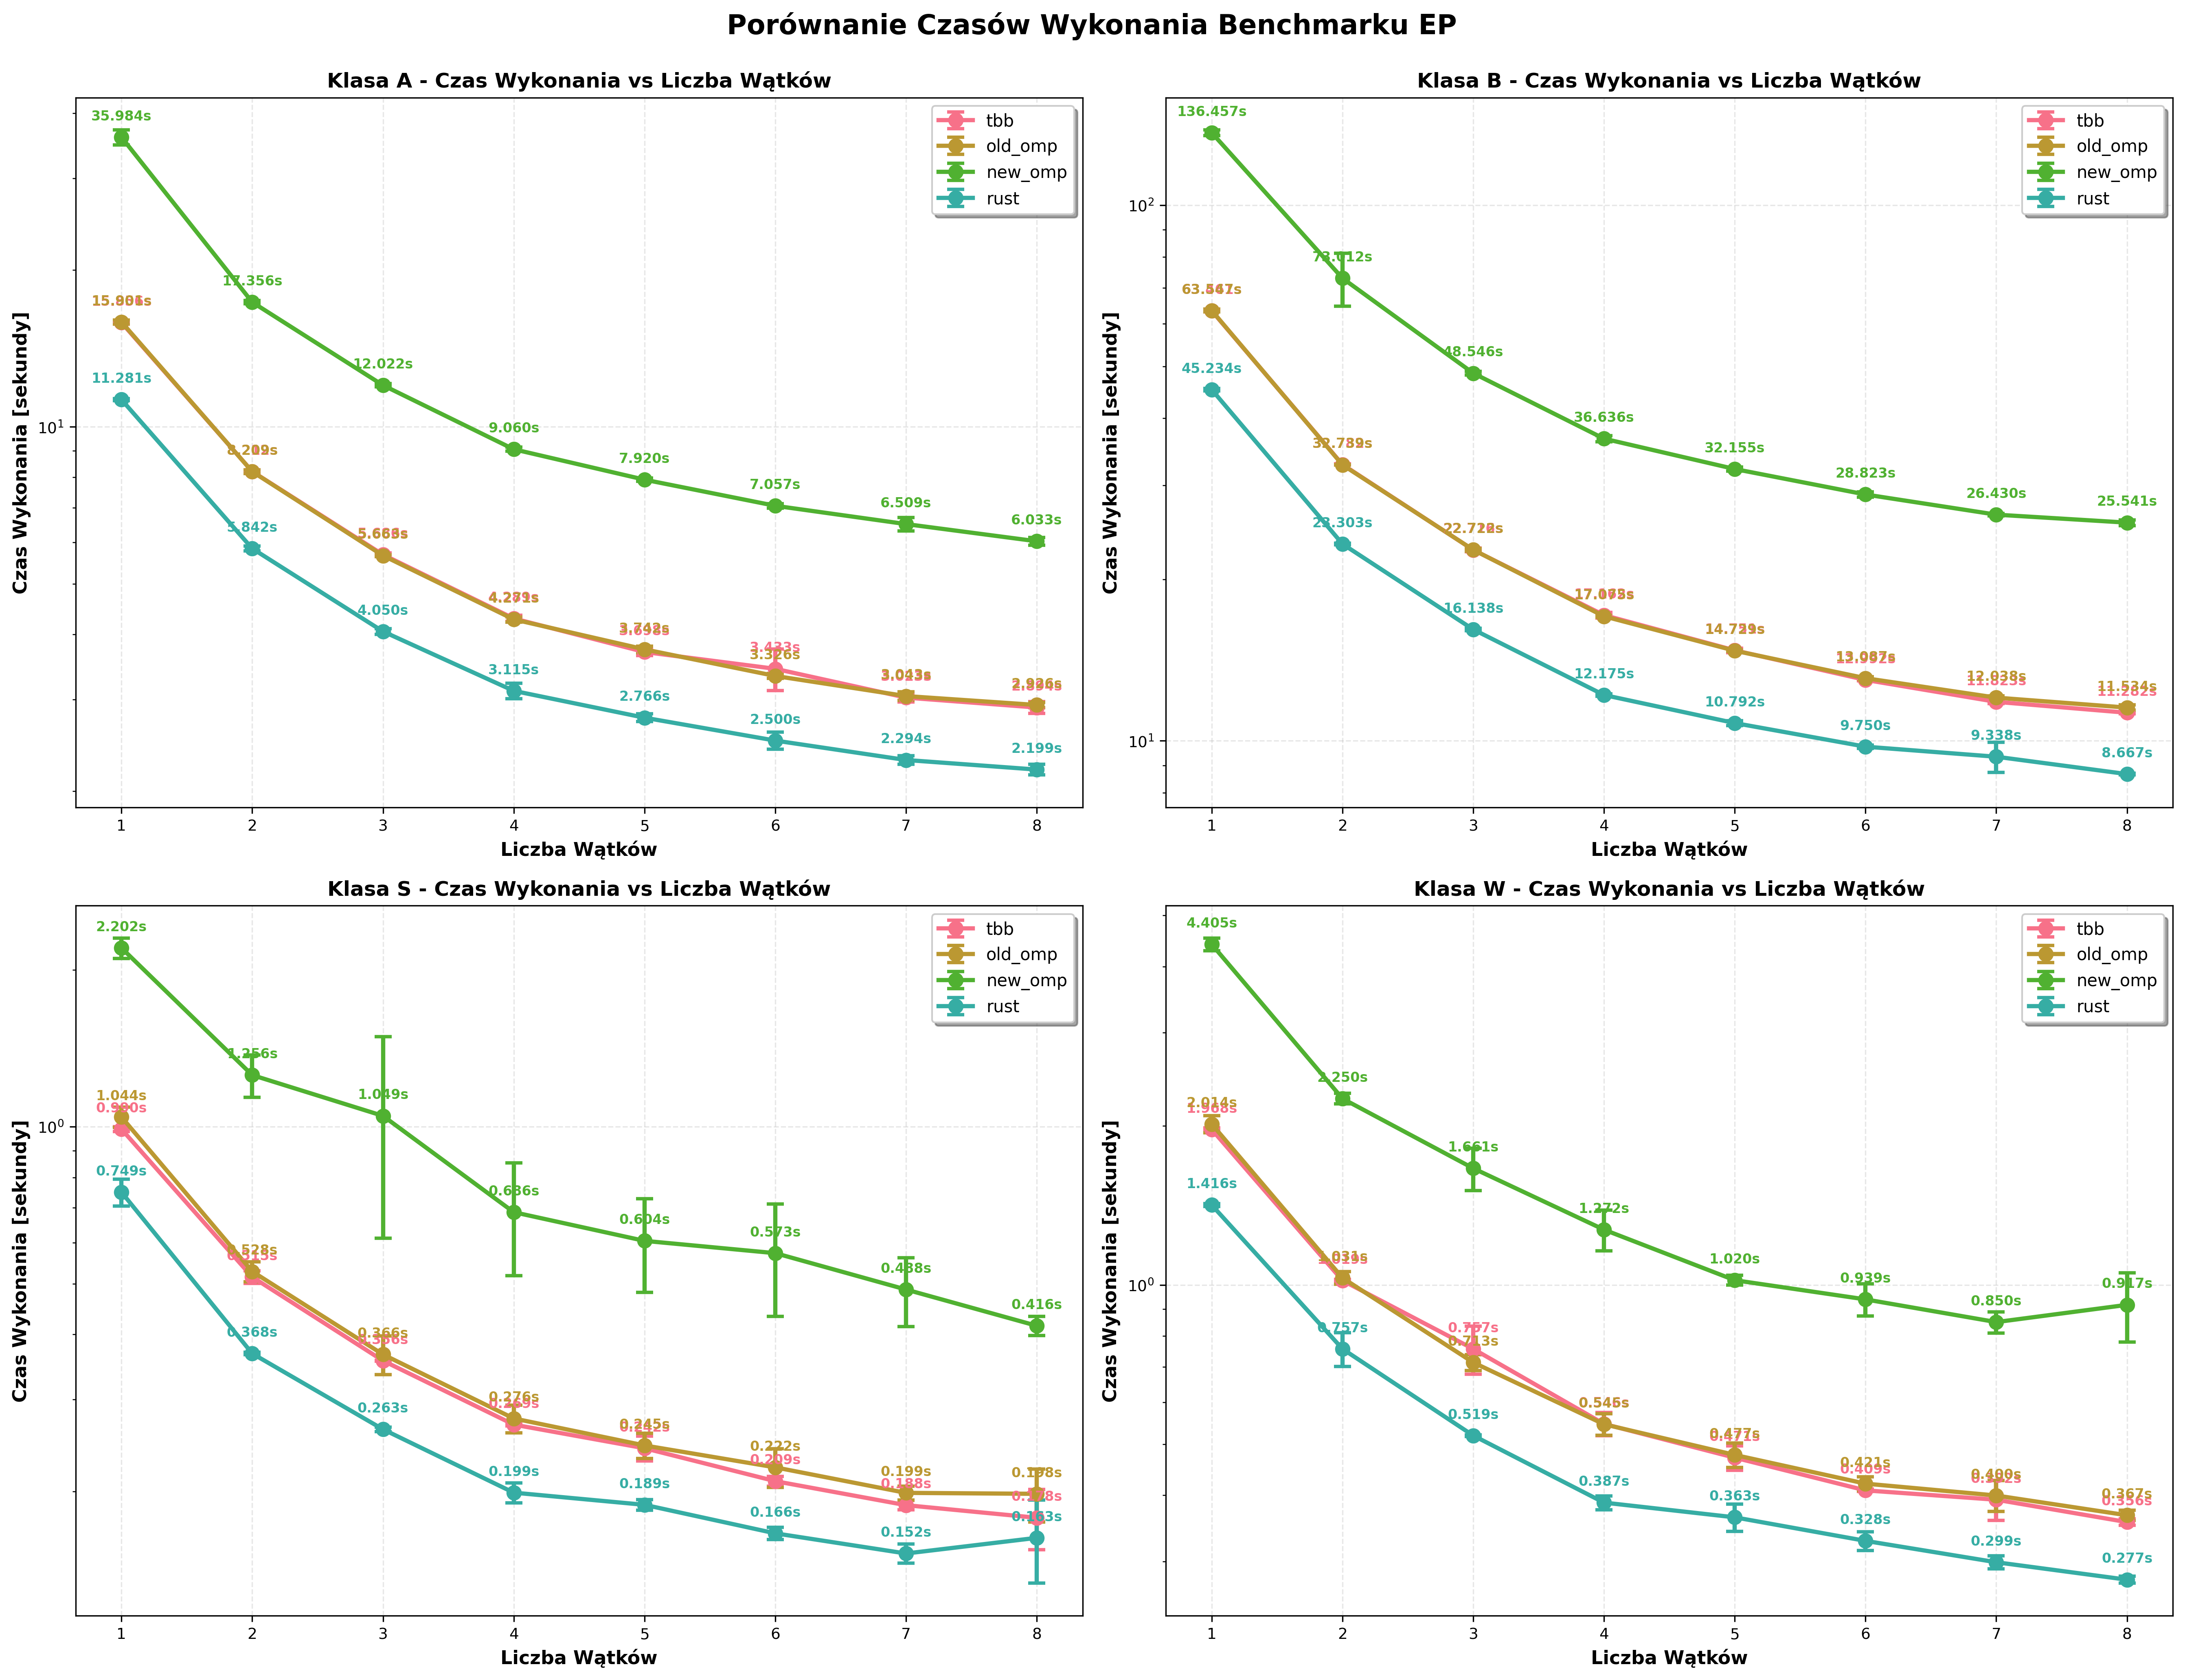
\includegraphics[width=\textwidth]{analiza/images/parallel/ep/ep_porownanie_czasow_wykonania.png}
    \caption{Porównanie czasów wykonania benchmarku EP dla klas S, W, A, B względem liczby użytych wątków}
    \label{ep_porownanie_czasow_wykonania}
\end{figure}

Na rysunku \ref{ep_porownanie_czasow_wykonania} zaprezentowano zestawienie czasów wykonania benchmarku EP dla czterech klas problemu: S, W, A oraz B, przy użyciu czterech różnych implementacji równoległości: TBB, OpenMP w wersji oryginalnej w stylu języka Fortran (old\_omp), OpenMP w wersji nowszej (new\_omp) oraz implementacji w języku Rust. Dla każdej z klas przedstawiono zależność czasu wykonania od liczby wątków (od 1 do 8). Wartości zostały zaprezentowane w skali logarytmicznej.

\begin{figure}[H]
    \centering
    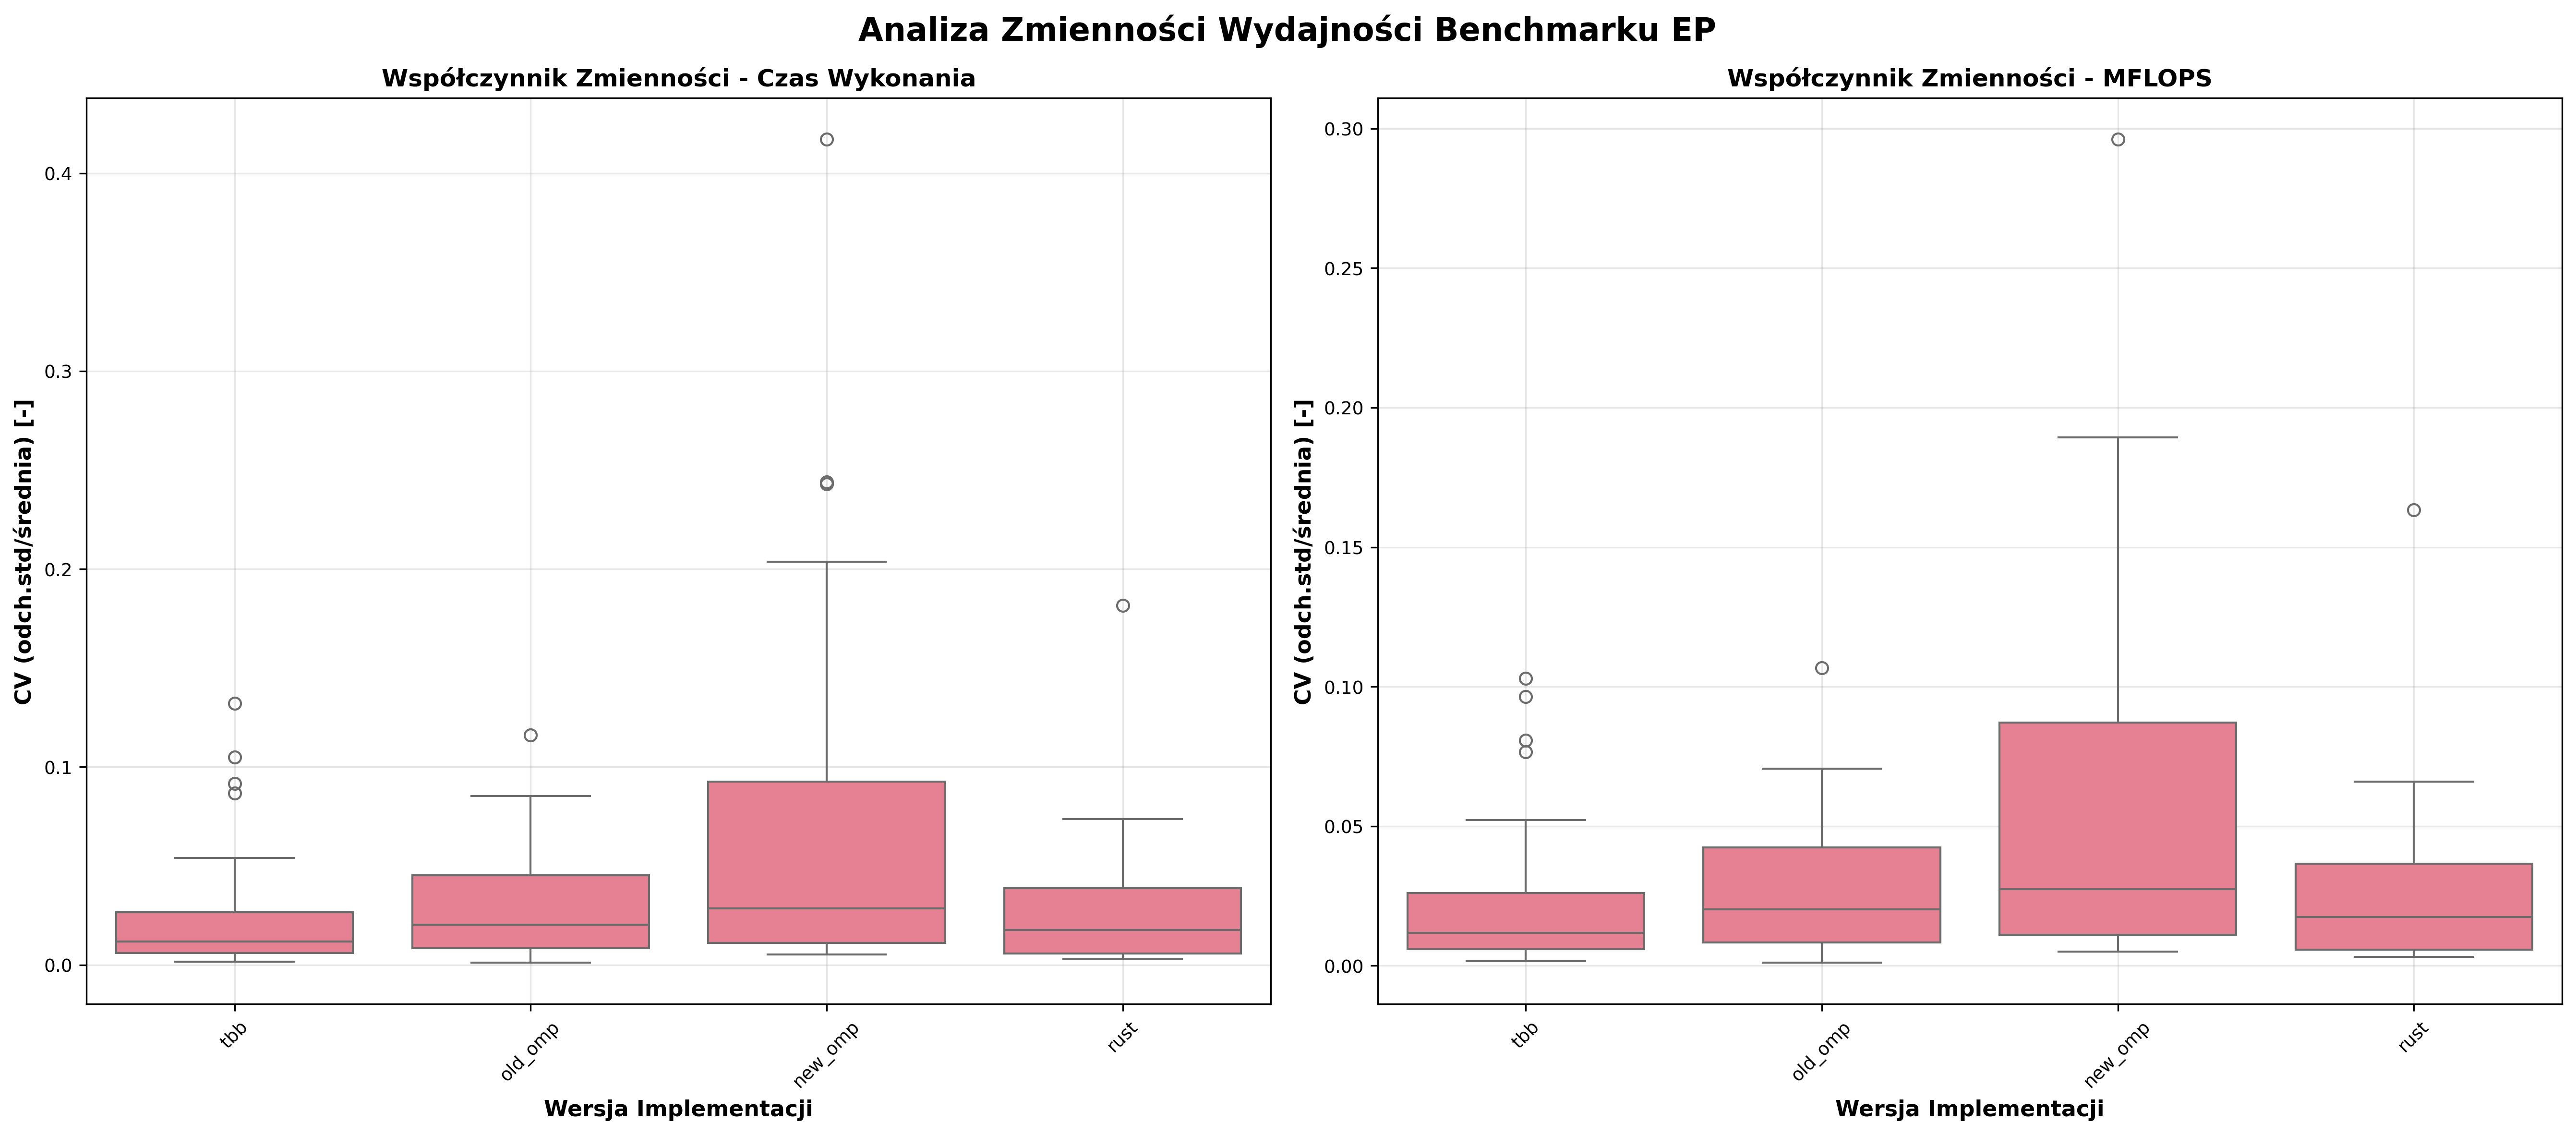
\includegraphics[width=\textwidth]{analiza/images/parallel/ep/ep_analiza_zmiennosci.png}
    \caption{Analiza zmienności czasów wykonania benchmarku EP dla klas S, W, A, B względem liczby użytych wątków}
    \label{ep_analiza_zmiennosci}
\end{figure}

Analizując czasy wykonania rysunki \ref{ep_porownanie_czasow_wykonania} oraz \ref{ep_analiza_zmiennosci} benchmarku EP dla czterech klas problemów (S, W, A, B), można zauważyć wyraźne różnice między poszczególnymi implementacjami wielowątkowymi. Najlepszą efektywność obliczeniową - mierzoną czasem wykonania - wykazuje new\_omp, która niezależnie od liczby wątków osiąga najniższe czasy w każdej z klas problemu. Jej wykresy cechują się systematycznym spadkiem czasu przy wzroście liczby wątków, co świadczy o bardzo dobrej skalowalności.

Implementacje tbb oraz old\_omp wykazują zbliżoną wydajność, nieco gorszą od new\_omp, ale znacząco lepszą od rust. Co istotne, rust osiąga zdecydowanie najdłuższe czasy wykonania, zwłaszcza dla dużych klas (A i B), gdzie jego możliwości skalowania są wyraźnie ograniczone. Pomimo to, rust zachowuje stabilność wyników i charakteryzuje się stosunkowo niską zmiennością pomiarów.

Potwierdza to analiza współczynnika zmienności \eng{Coefficient of Variation, CV} \ref{ep_analiza_zmiennosci}, przedstawiona na wykresie pudełkowym. Współczynnik ten jest liczony jako stosunek odchylenia standardowego do średniej wartości, co pozwala ocenić relatywną stabilność wyników:
\begin{itemize}
    \item czas wykonania (lewy wykres): tbb, old\_omp i rust wykazują niskie wartości CV, co oznacza wysoką powtarzalność czasów wykonania. new\_omp, mimo najlepszych wyników wydajnościowych, cechuje się większą zmiennością - w skrajnych przypadkach CV sięga powyżej 0.4, co może sugerować podatność na wahania warunków systemowych lub efekt optymalizacji niejednorodnych dla różnych klas danych.
    \item MFLOPS (prawy wykres): Wskaźniki zmienności osiągają podobny charakter, gdzie tbb i rust są najstabilniejsze, zaś new\_omp posiada najwyższe wartości rozrzutu, potwierdzające większą niestabilność w osiąganych wynikach liczbowych, mimo wysokiej wydajności średniej.
\end{itemize}


%------------------------------
\begin{figure}[H]
    \centering
    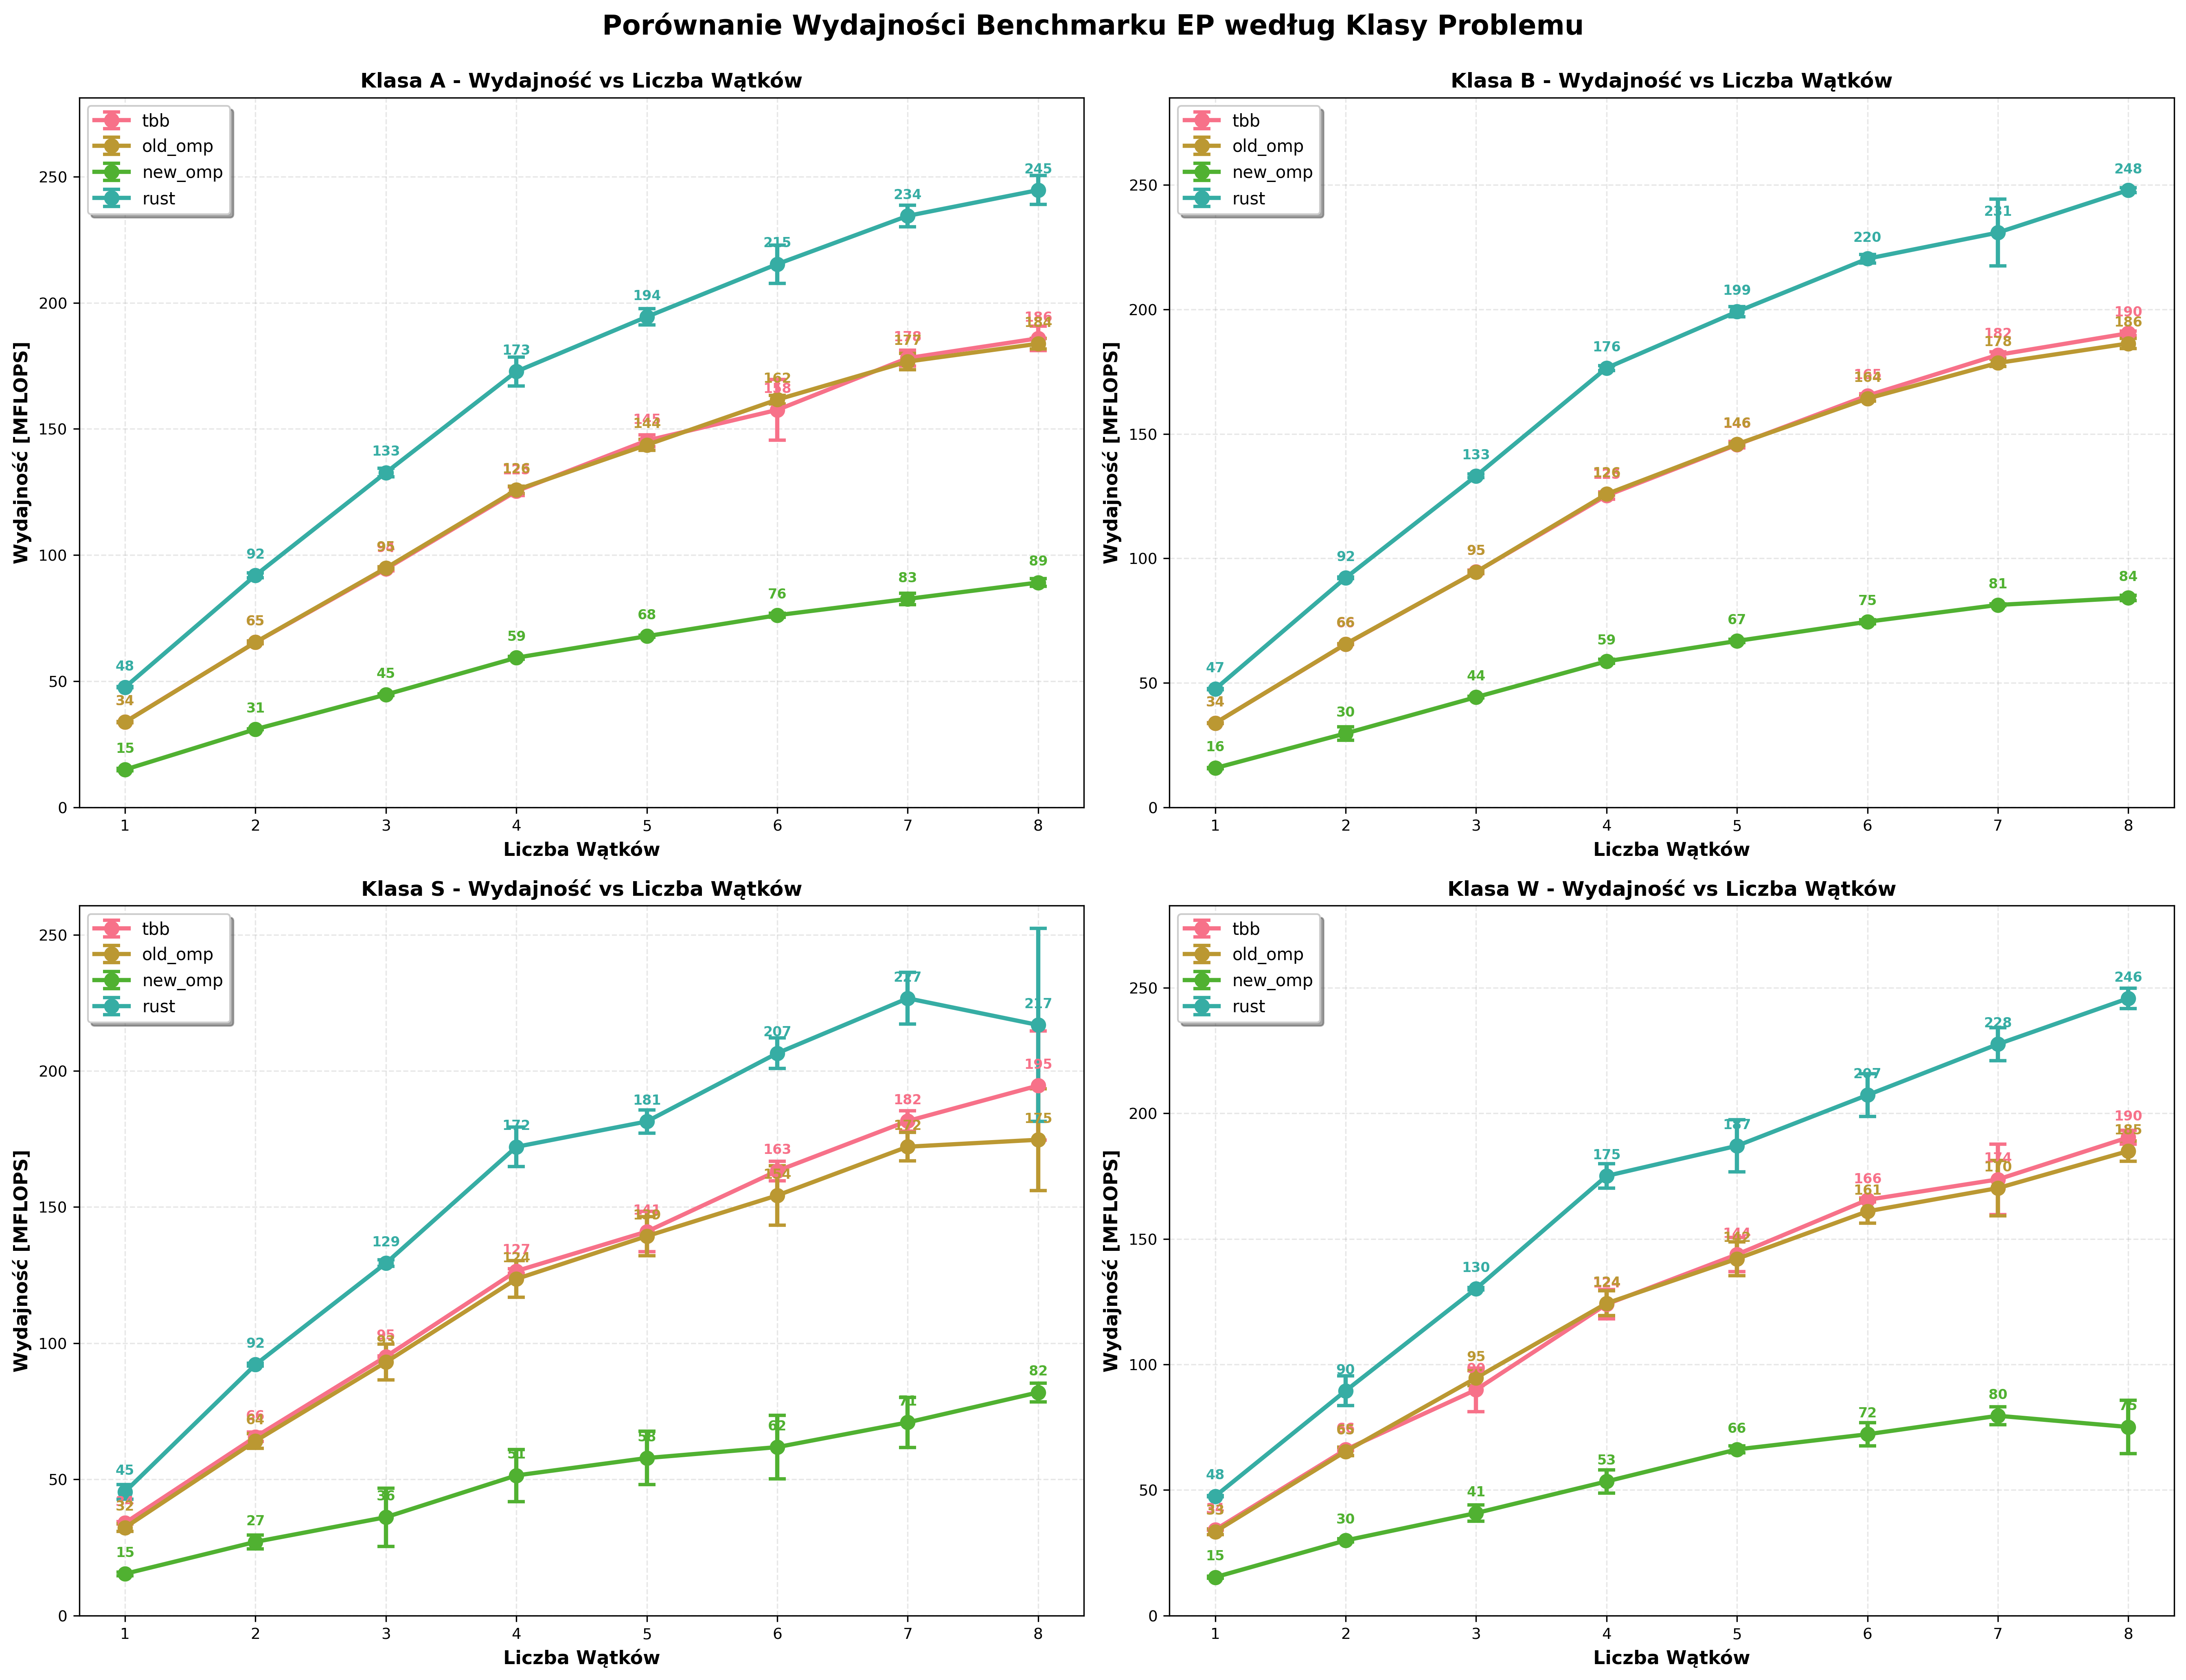
\includegraphics[width=\textwidth]{analiza/images/parallel/ep/ep_porownanie_wydajnosci.png}
    \caption{Porównanie wydajności benchmarku EP dla klas S, W, A, B względem liczby użytych wątków}
    \label{ep_porownanie_wydajnosci}
\end{figure}
Na wykresach na rysunku \ref{ep_porownanie_wydajnosci} zaprezentowano porównanie wydajności benchmarku EP mierzonej w MFLOPS (milionach operacji zmiennoprzecinkowych na sekundę). Wydajność została przedstawiona jako funkcja liczby wątków (1-8) dla czterech implementacji równoległych.

Wraz ze wzrostem klasy problemu (czyli rozmiaru danych wejściowych), wzrastają również bezwzględne wartości MFLOPS osiągane przez każdą z implementacji. Jest to zgodne z oczekiwaniami dla benchmarków typu EP, w których większe rozmiary problemu pozwalają efektywniej ukrywać narzut związany z zarządzaniem równoległością.
\begin{itemize}
    \item klasa B pozwala najlepiej uwidocznić różnice między implementacjami, dając największe zróżnicowanie MFLOPS przy 8 wątkach,
    \item klasy S i W, będące mniejszymi pod względem danych, charakteryzują się mniejszymi wartościami bezwzględnymi MFLOPS i niższym przyrostem przy zwiększaniu liczby wątków.
    \item rust osiąga najniższe wartości MFLOPS w każdej z klas, nawet przy wysokiej liczbie wątków. Dla klasy B i 8 wątków osiąga zaledwie 84 MFLOPS, co sugeruje istotne ograniczenia w implementacji mechanizmu równoległości. Niemniej jednak, krzywa wzrostu jest regularna, co może świadczyć o poprawnie działającej, choć mniej zoptymalizowanej strategii równoległości.
\end{itemize}





\begin{figure}[H]
    \centering
    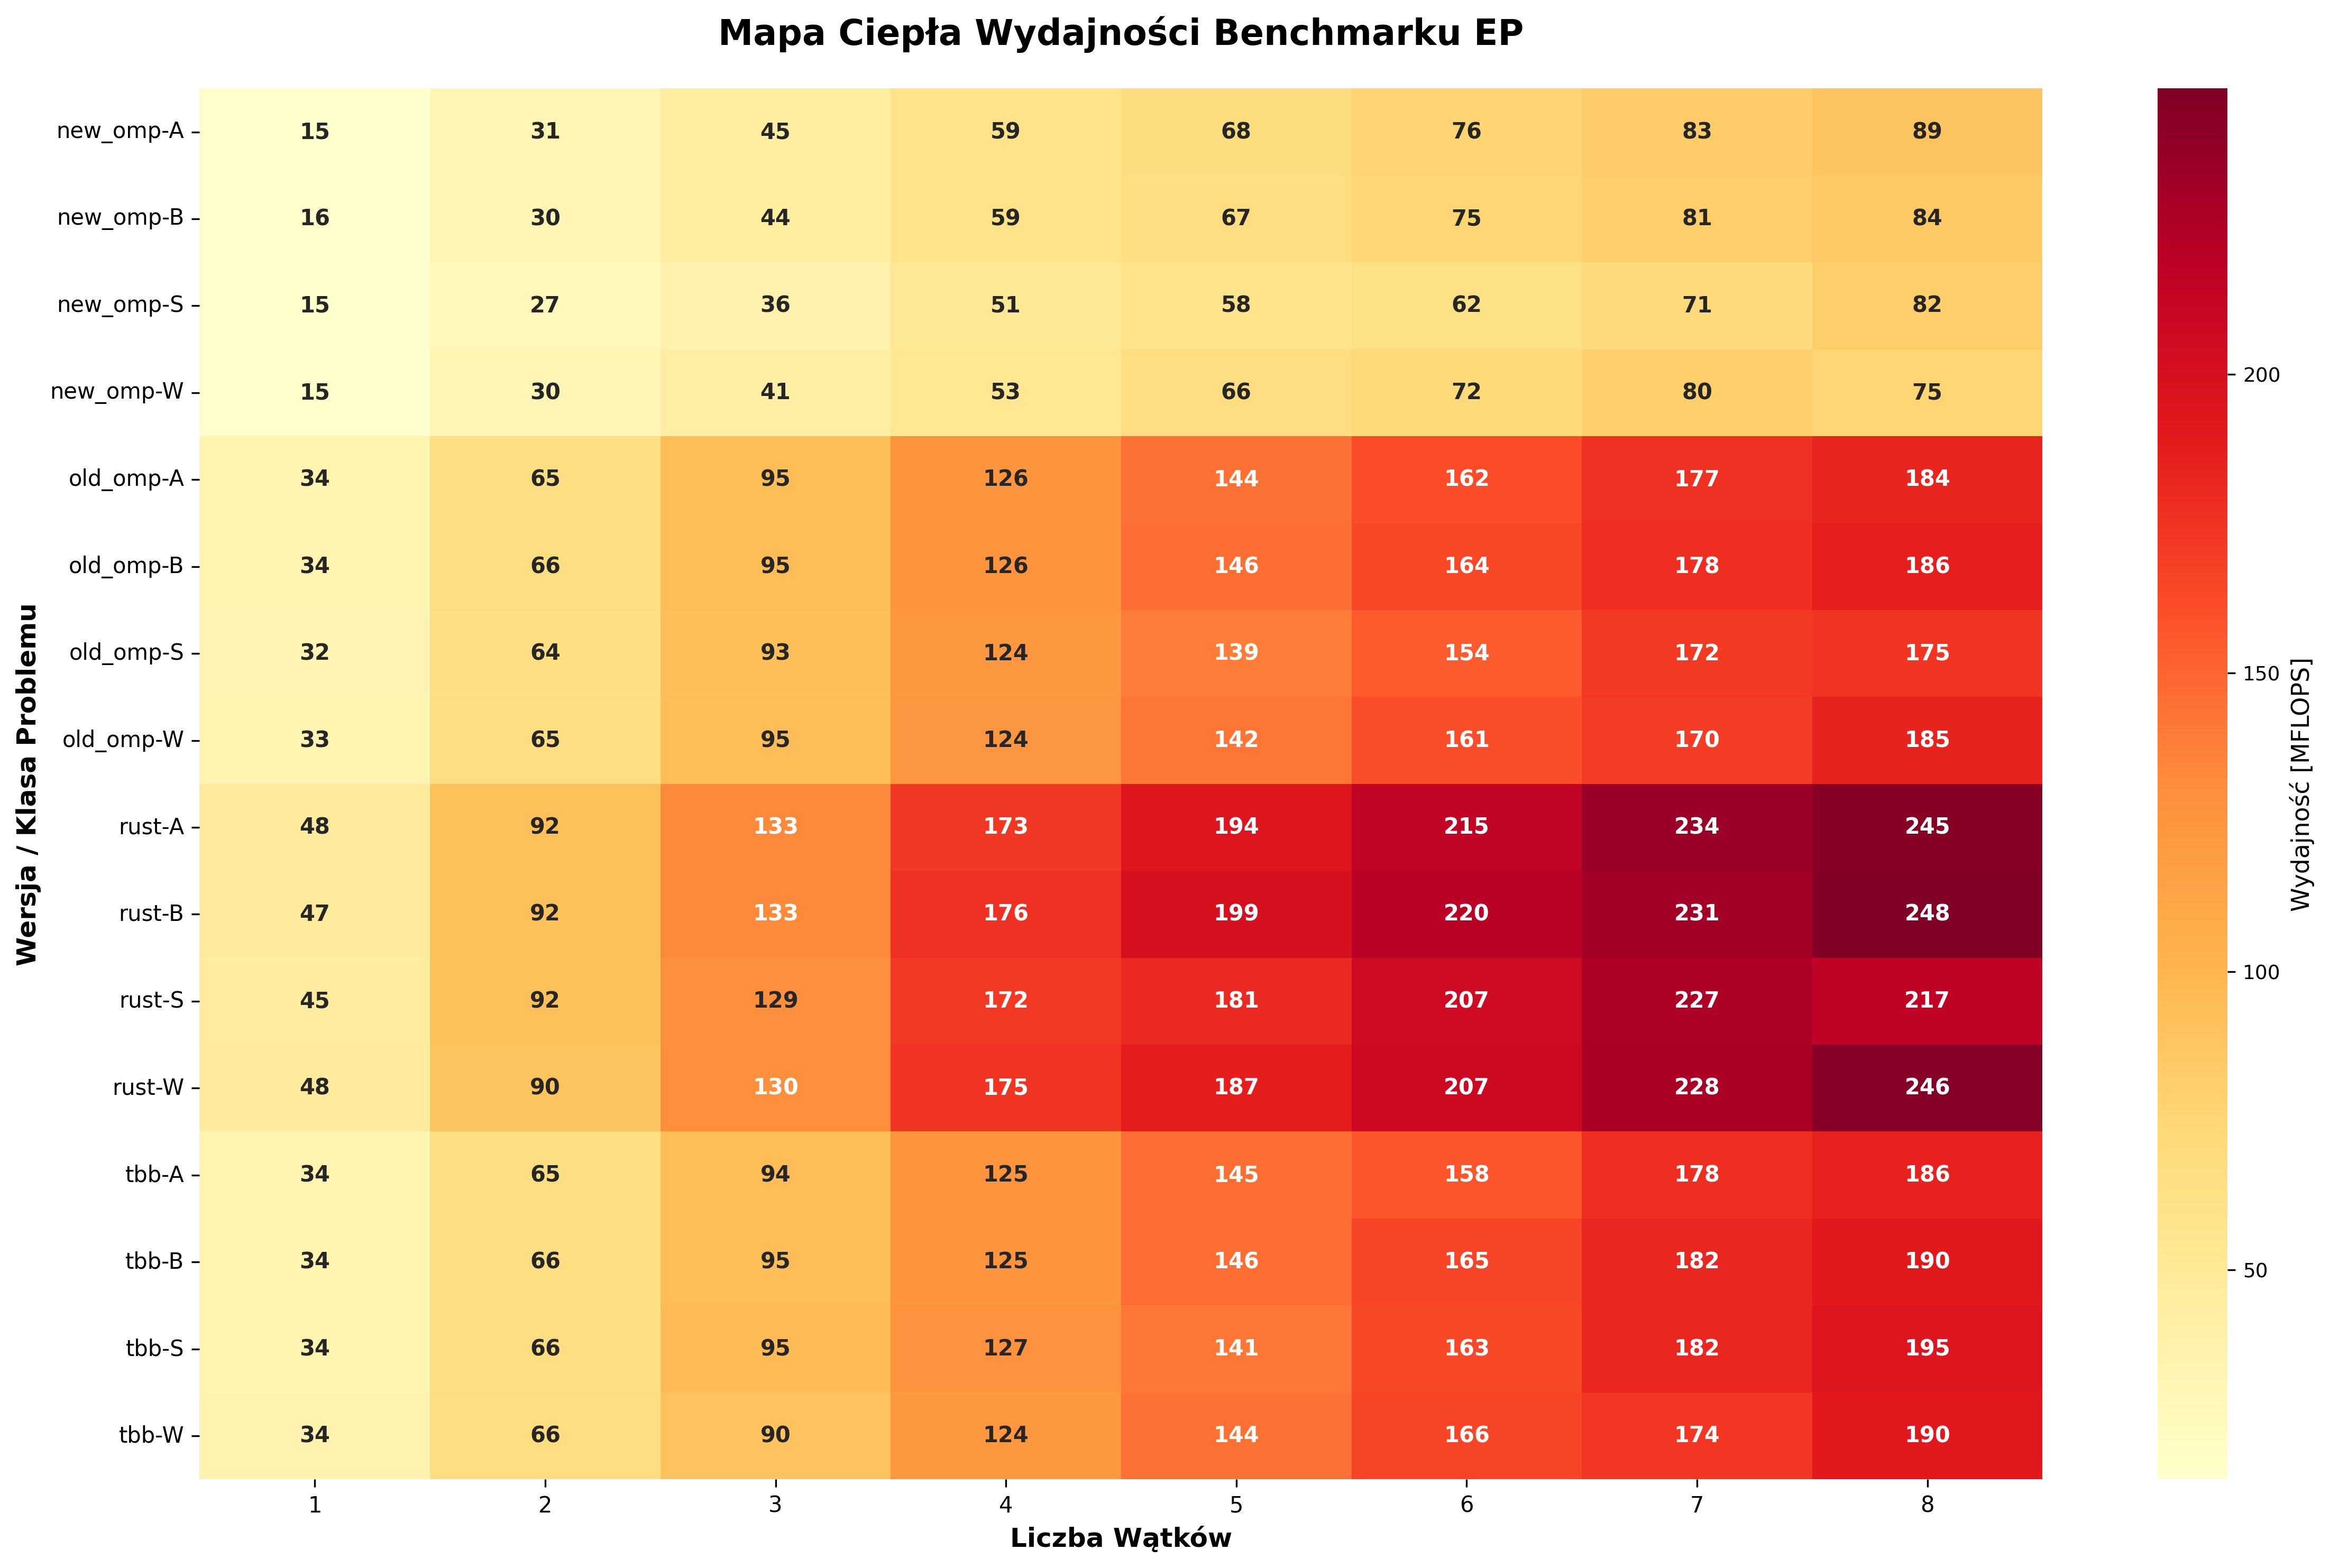
\includegraphics[width=\textwidth]{analiza/images/parallel/ep/ep_mapa_ciepla_wydajnosci.png}
    \caption{Mapa ciepła wydajności benchmarku EP dla klas S, W, A, B względem liczby użytych wątków}
    \label{ep_heatmap_wydajnosci}
\end{figure}
Powyższa mapa cieplna - rysunek \ref{ep_heatmap_wydajnosci} przedstawia wydajność (w MFLOPS). Wydajność została przedstawiona w zależności od liczby użytych wątków. Odcienie koloru od żółtego do ciemnoczerwonego wskazują na wzrost wydajności.
Mapa cieplna potwierdza dane z wykresów liniowych \ref{ep_porownanie_wydajnosci}, dając jednocześnie szybki przegląd przekrojowy:
\begin{itemize}
    \item największe wartości wydajności skoncentrowane są w implementacjach new\_omp i old\_omp, przy największych klasach i liczbie wątków,
    \item tbb zachowuje dużą spójność między klasami problemu, co może wskazywać na dobrą przenośność implementacji,
    \item rust zaskakuje wysokimi wartościami bazowymi (dla 1-2 wątków), jednak jego krzywa wzrostu MFLOPS szybko się wypłaszcza.
\end{itemize}





\begin{figure}[H]
    \centering
    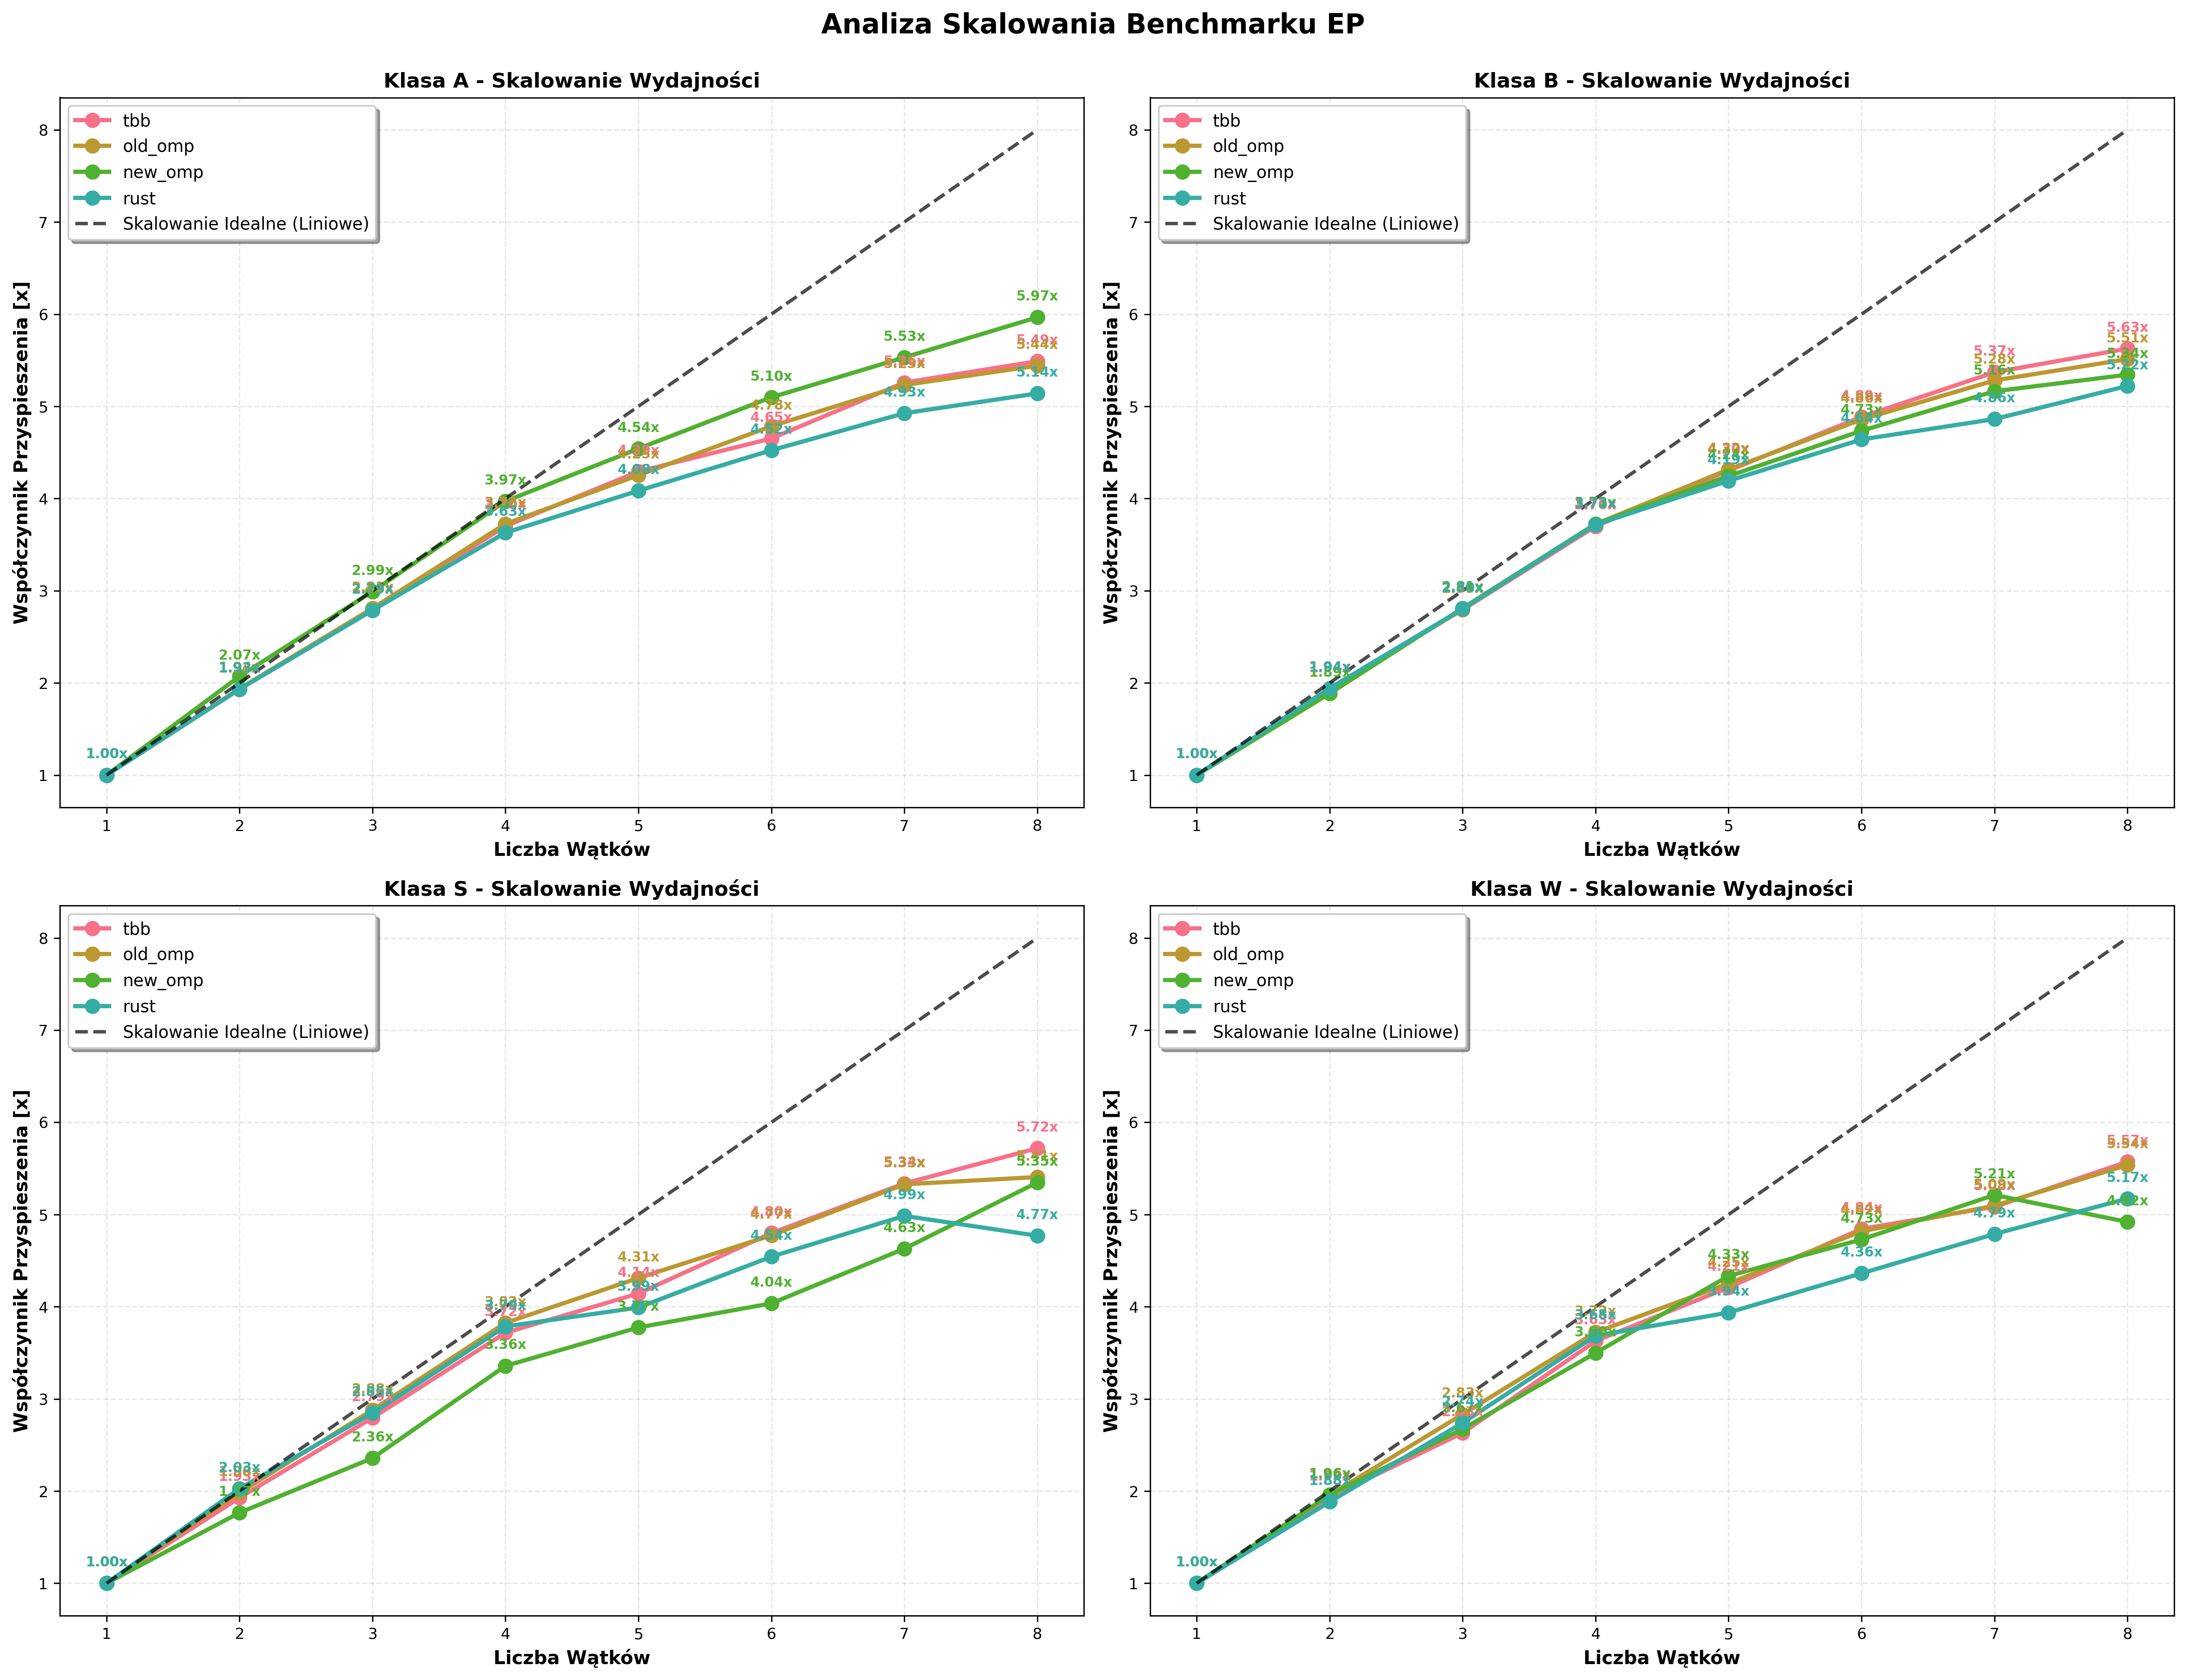
\includegraphics[width=\textwidth]{analiza/images/parallel/ep/ep_analiza_skalowania.png}
    \caption{Analiza skalowania benchmarku EP dla klas S, W, A, B względem liczby użytych wątków}
    \label{ep_analiza_skalowania}
\end{figure}
Powyższy wykres - rysunek \ref{ep_analiza_skalowania} przedstawia skalowanie wydajności benchmarku EP. Skalowanie wyrażone zostało za pomocą współczynnika przyspieszenia względem wykonania jednowątkowego i odniesione do skalowania idealnego (liniowego).
Wszystkie implementacje wykazują niemal liniowy wzrost do 4 wątków. Po tym punkcie zaczyna być widoczne stopniowe wypłaszczanie krzywych przyrostu, co może wynikać z:
\begin{itemize}
    \item ograniczeń sprzętowych (np. architektura procesora),
    \item narzutu synchronizacji,
    \item efektu wyczerpania równoległości w algorytmie EP - prawo Amdahla.
\end{itemize}


\subsection{Wyniki benchmarków - platforma x86\_64}
%------------------------------
%------------------------------

\subsection{Wyniki profilowania wydajności - platforma ARM64}
W celu kompleksowego porównania efektywności testowanych implementacji benchmarku EP na platformie ARM64 dokonano analizy metryk systemowych dotyczących zarządzania pamięcią: zużycia pamięci \eng{memory usage}, liczby odzyskanych stron pamięci \eng{page reclaims}, liczby błędów stron pamięci \eng{page faults} oraz ich wzajemnych relacji.
\begin{figure}[H]
    \centering
    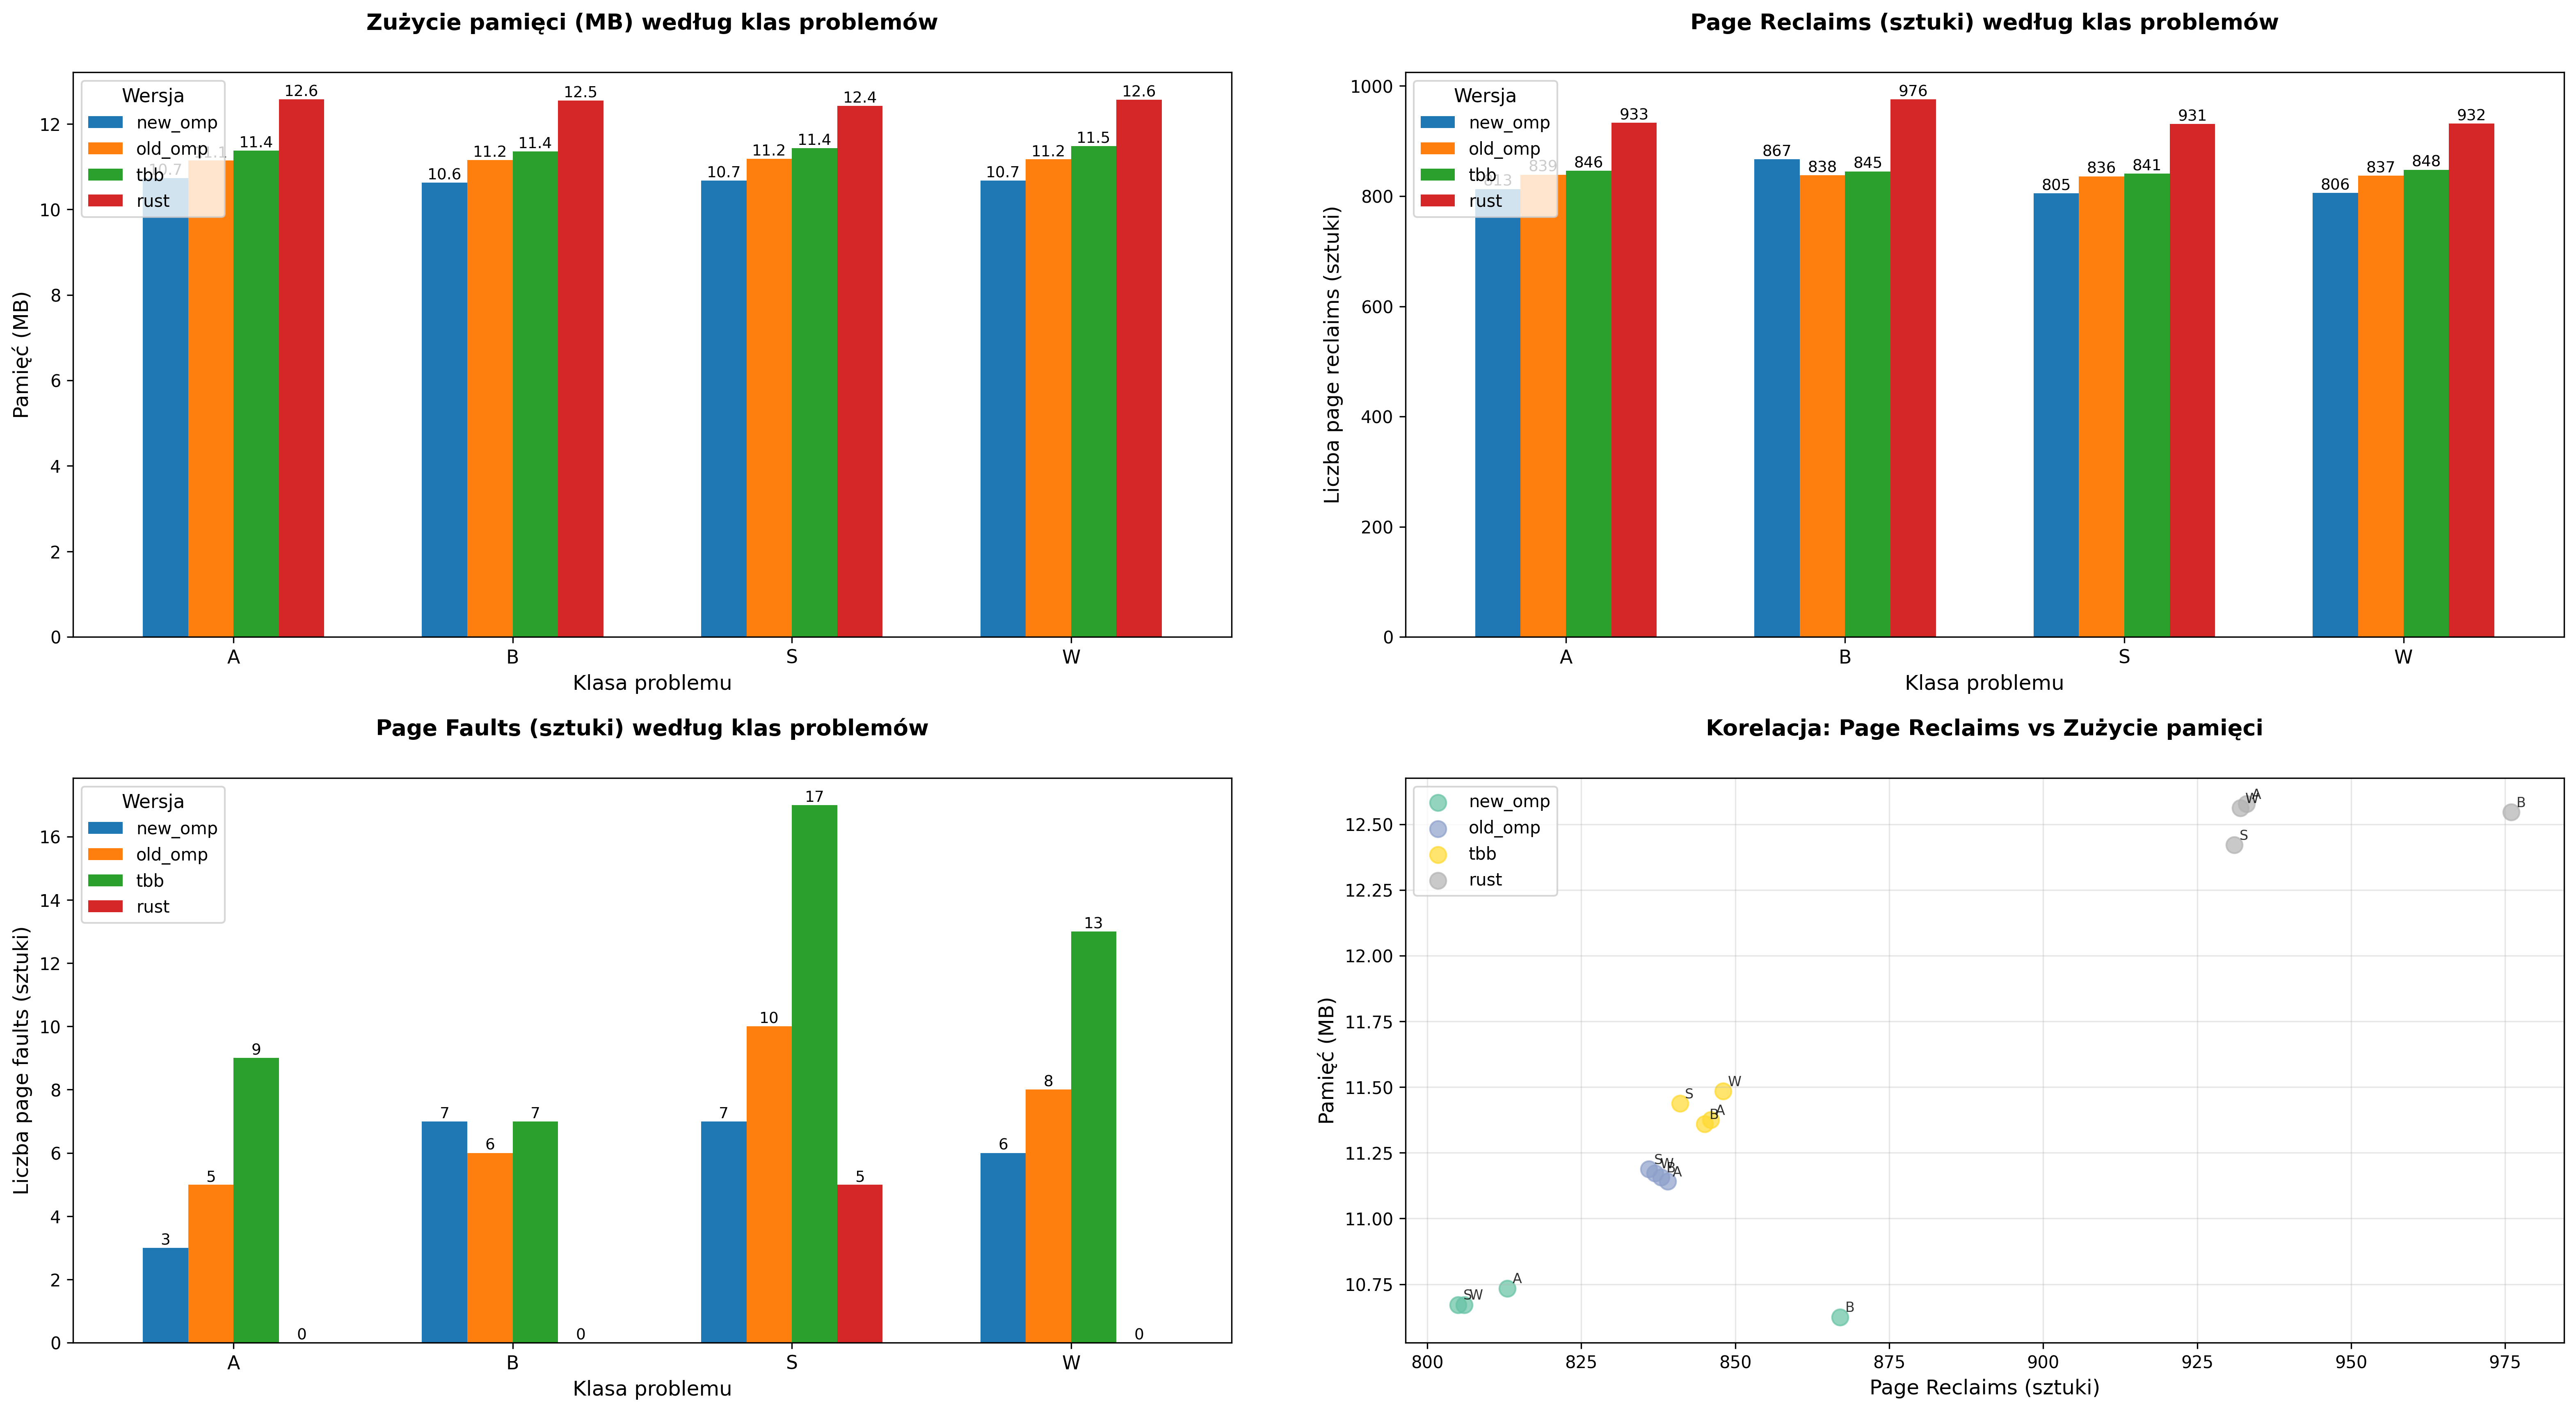
\includegraphics[width=\textwidth]{analiza/images/parallel/ep/chart_01_memory_comparison.png}
    \caption{Profilowanie wydajności benchmarku EP dla klas S, W, A, B względem liczby użytych wątków}
    \label{ep_porownanie_zuzycia_pamieci}
\end{figure}
 
\subsubsection{Zużycie pamięci i  liczba odzyskanych stron}
W górnym wierszu rysunku \ref{ep_porownanie_zuzycia_pamieci} przedstawiono bezwzględne zużycie pamięci oraz liczbę odzyskanych stron pamięci dla każdej klasy problemu. Analiza pokazuje, że implementacje new\_omp oraz tbb charakteryzują się najniższym zużyciem pamięci, utrzymując wartości w przedziale 10,6-11,2 MB. Z kolei rust oraz old\_omp wykazują nieco wyższe zużycie (do 12,6 MB), przy czym rust w każdej klasie wykorzystuje więcej pamięci niż tbb.

Liczba odzyskanych stron pozostaje względnie stabilna między klasami i wersjami, oscylując w granicach 800-970, z najwyższymi wartościami przypadającymi na rust, co może wskazywać na intensywne operacje zarządzania pamięcią (przydziały i zwolnienia stron).

\subsubsection{Błędy stron pamięci oraz korelacja}
Liczba błędów stron najniższa była dla rust, gdzie w klasach B i W całkowicie je wyeliminowano. new\_omp oraz old\_omp wykazują umiarkowaną liczbę błędów, natomiast najwyższe wartości błędów występują dla tbb, osiągając aż 17 błędów w klasie S. Taki rozrzut może wskazywać na różne strategie zarządzania pamięcią oraz różne podejścia do alokacji dynamicznej.

Wykres korelacyjny w prawym dolnym rogu przedstawia związek między liczbą odzyskanych stron pamięci a zużyciem pamięci. Widoczna jest dodatnia korelacja między tymi metrykami, szczególnie wyraźna w przypadku rust, co potwierdza większą aktywność systemu zarządzania pamięcią tej implementacji.

\begin{figure}[H]
    \centering
    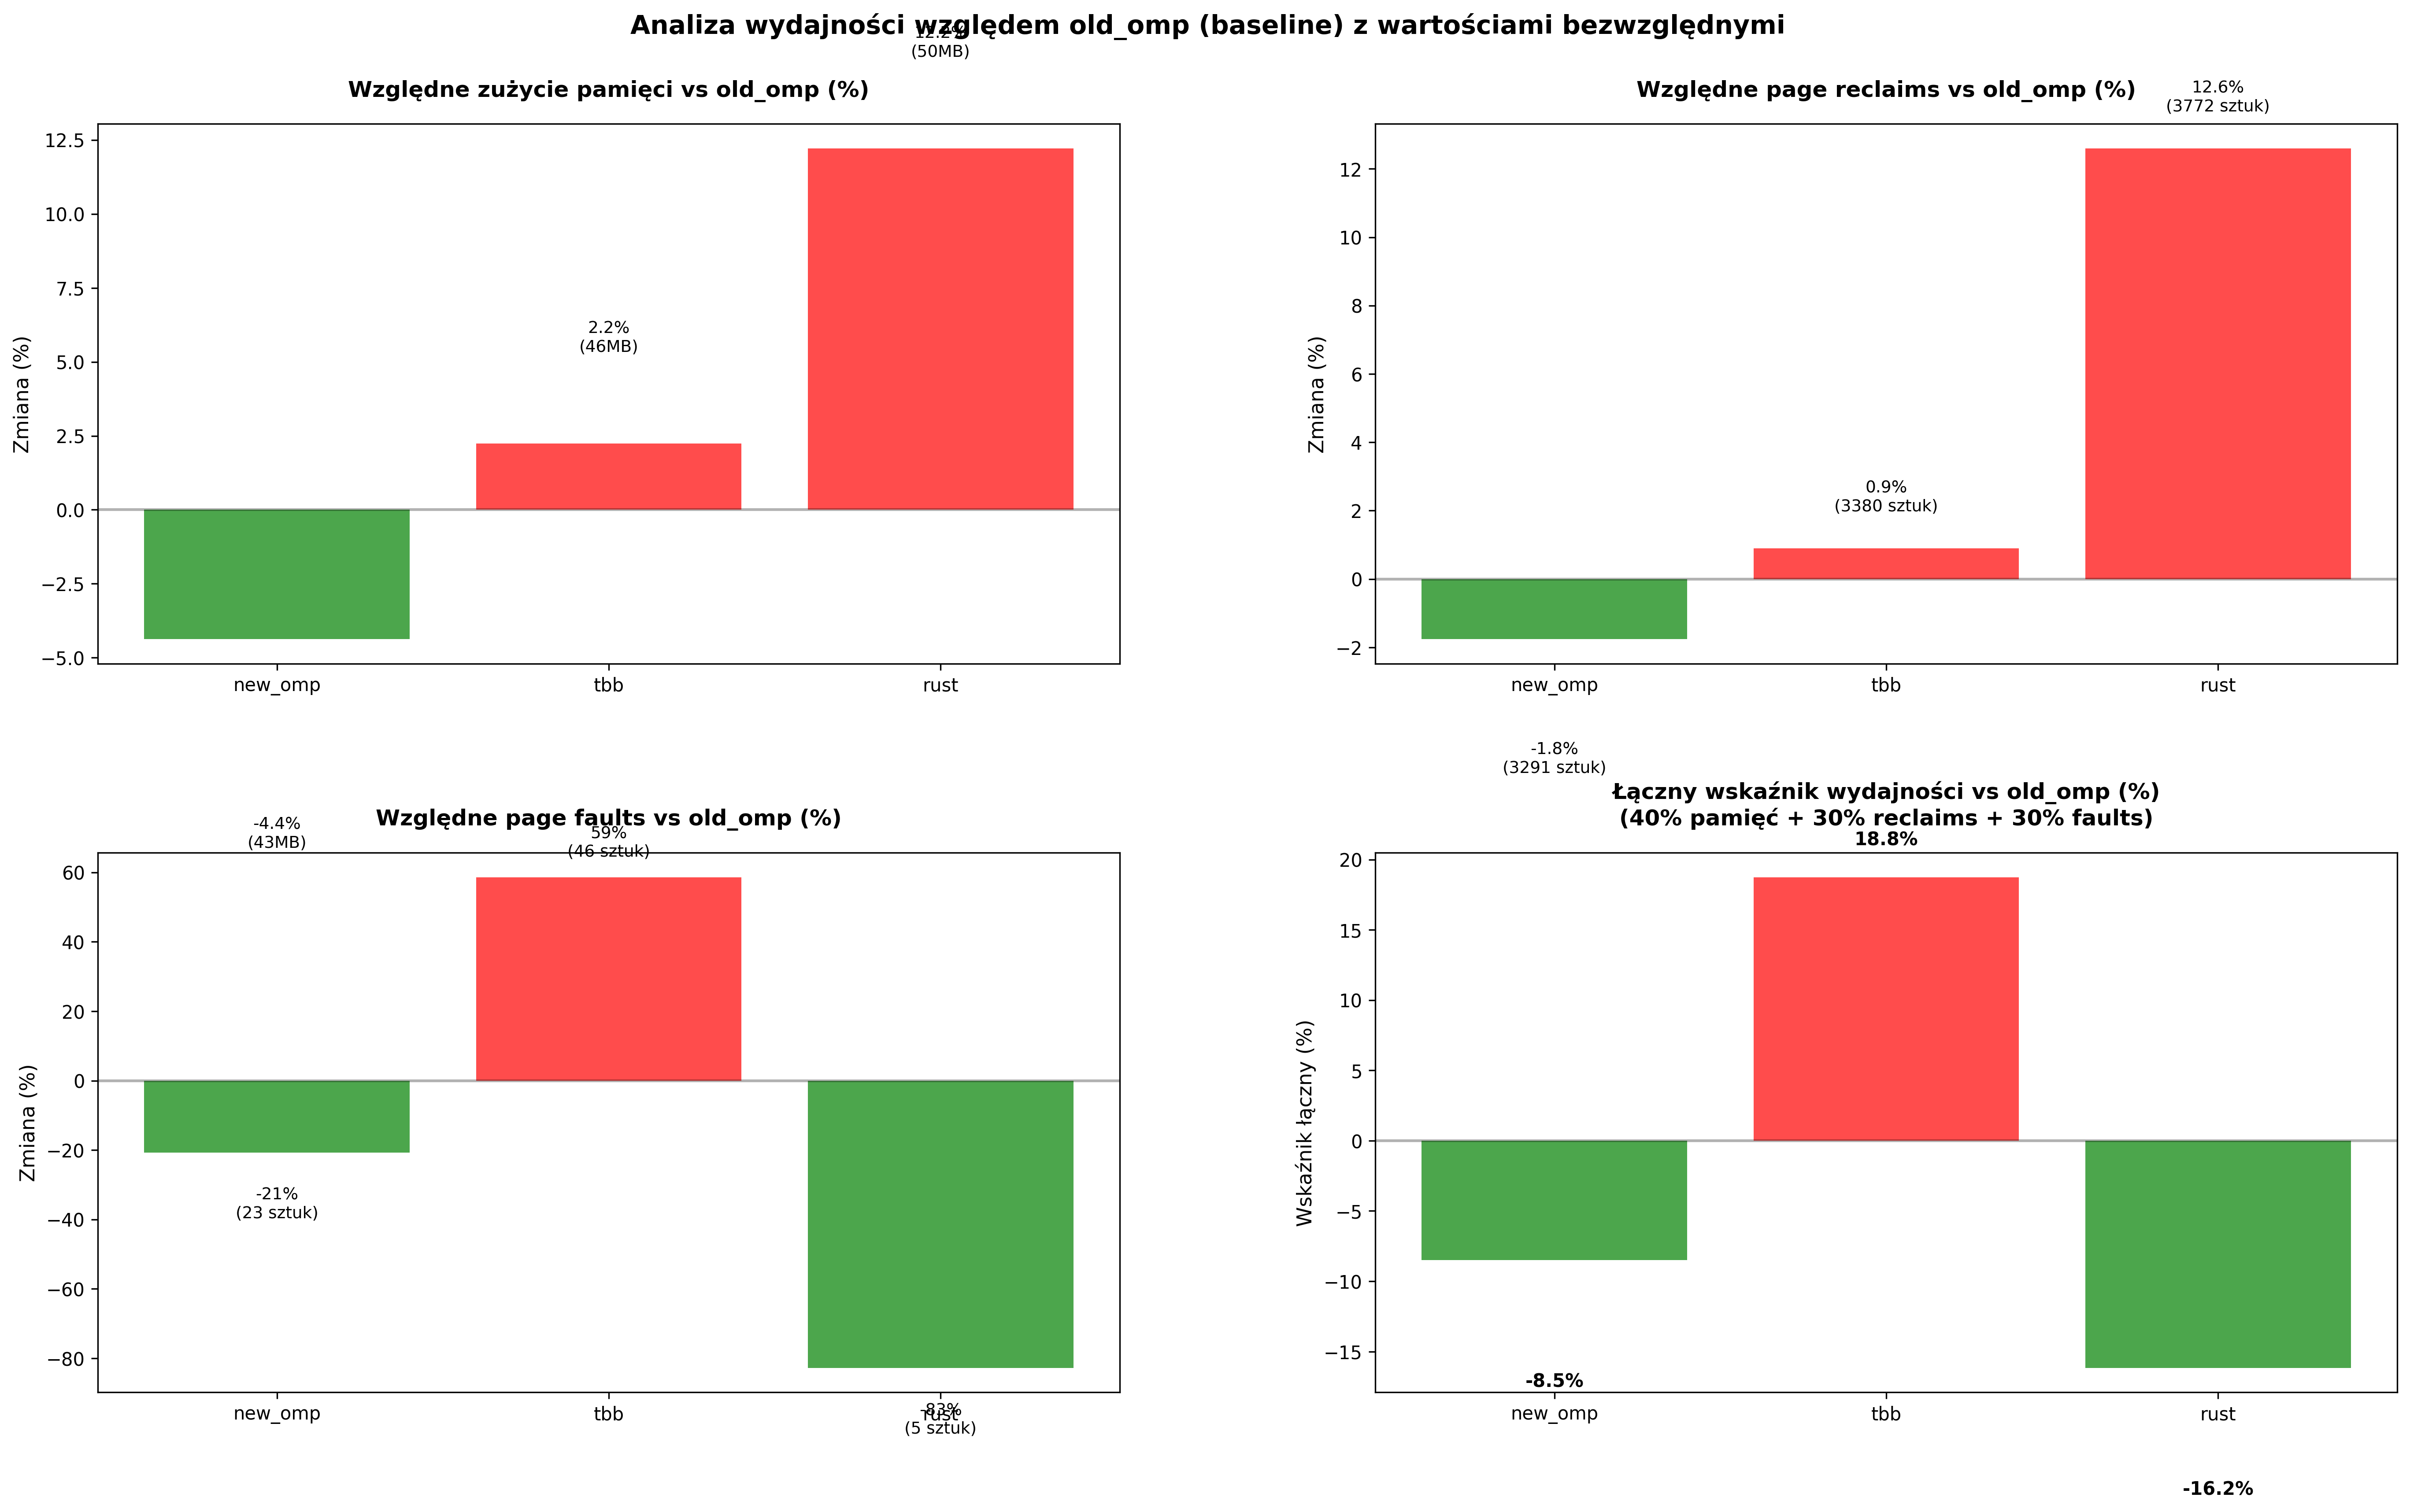
\includegraphics[width=\textwidth]{analiza/images/parallel/ep/chart_05_performance_ratios.png}
    \caption{Analiza wydajności względem old\_omp (punkt odniesienia) z wartościami bezwzględnymi}
    \label{ep_analiza_wzgledem_old_omp}
\end{figure}
Na rysunku \ref{ep_analiza_wzgledem_old_omp} zestawiono zmiany procentowe trzech analizowanych wskaźników względem implementacji referencyjnej old\_omp. Wskaźnikiem syntetycznym jest łączna metryka złożona z ważonych proporcji zużycia pamięci (40\%), zwolnionych stron (30\%) i błędów stron (30\%).
\begin{itemize}
    \item new\_omp uzyskał najniższe zużycie pamięci (-4,4\%) oraz najniższą liczbę page faults (-21\%), co złożyło się na końcowy wynik -8,5\% względem old\_omp.
    \item tbb, pomimo podobnego zużycia pamięci, odnotował wzrost błędów stron (59\%), co pogorszyło jego wynik ogólny (+18,8\%).
    \item rust, choć wyeliminował całkowicie błędy stron, jednocześnie cechował się najwyższym zużyciem pamięci i największą liczbą page reclaims (+12,6\%), co skutkowało końcowym wskaźnikiem -16,2\%.
\end{itemize}
Tym samym implementacja rust okazuje się najbardziej oszczędna pod względem zarządzania błędami stron, ale mniej efektywna pod względem ogólnego zarządzania pamięcią.



\begin{figure}[H]
    \centering
    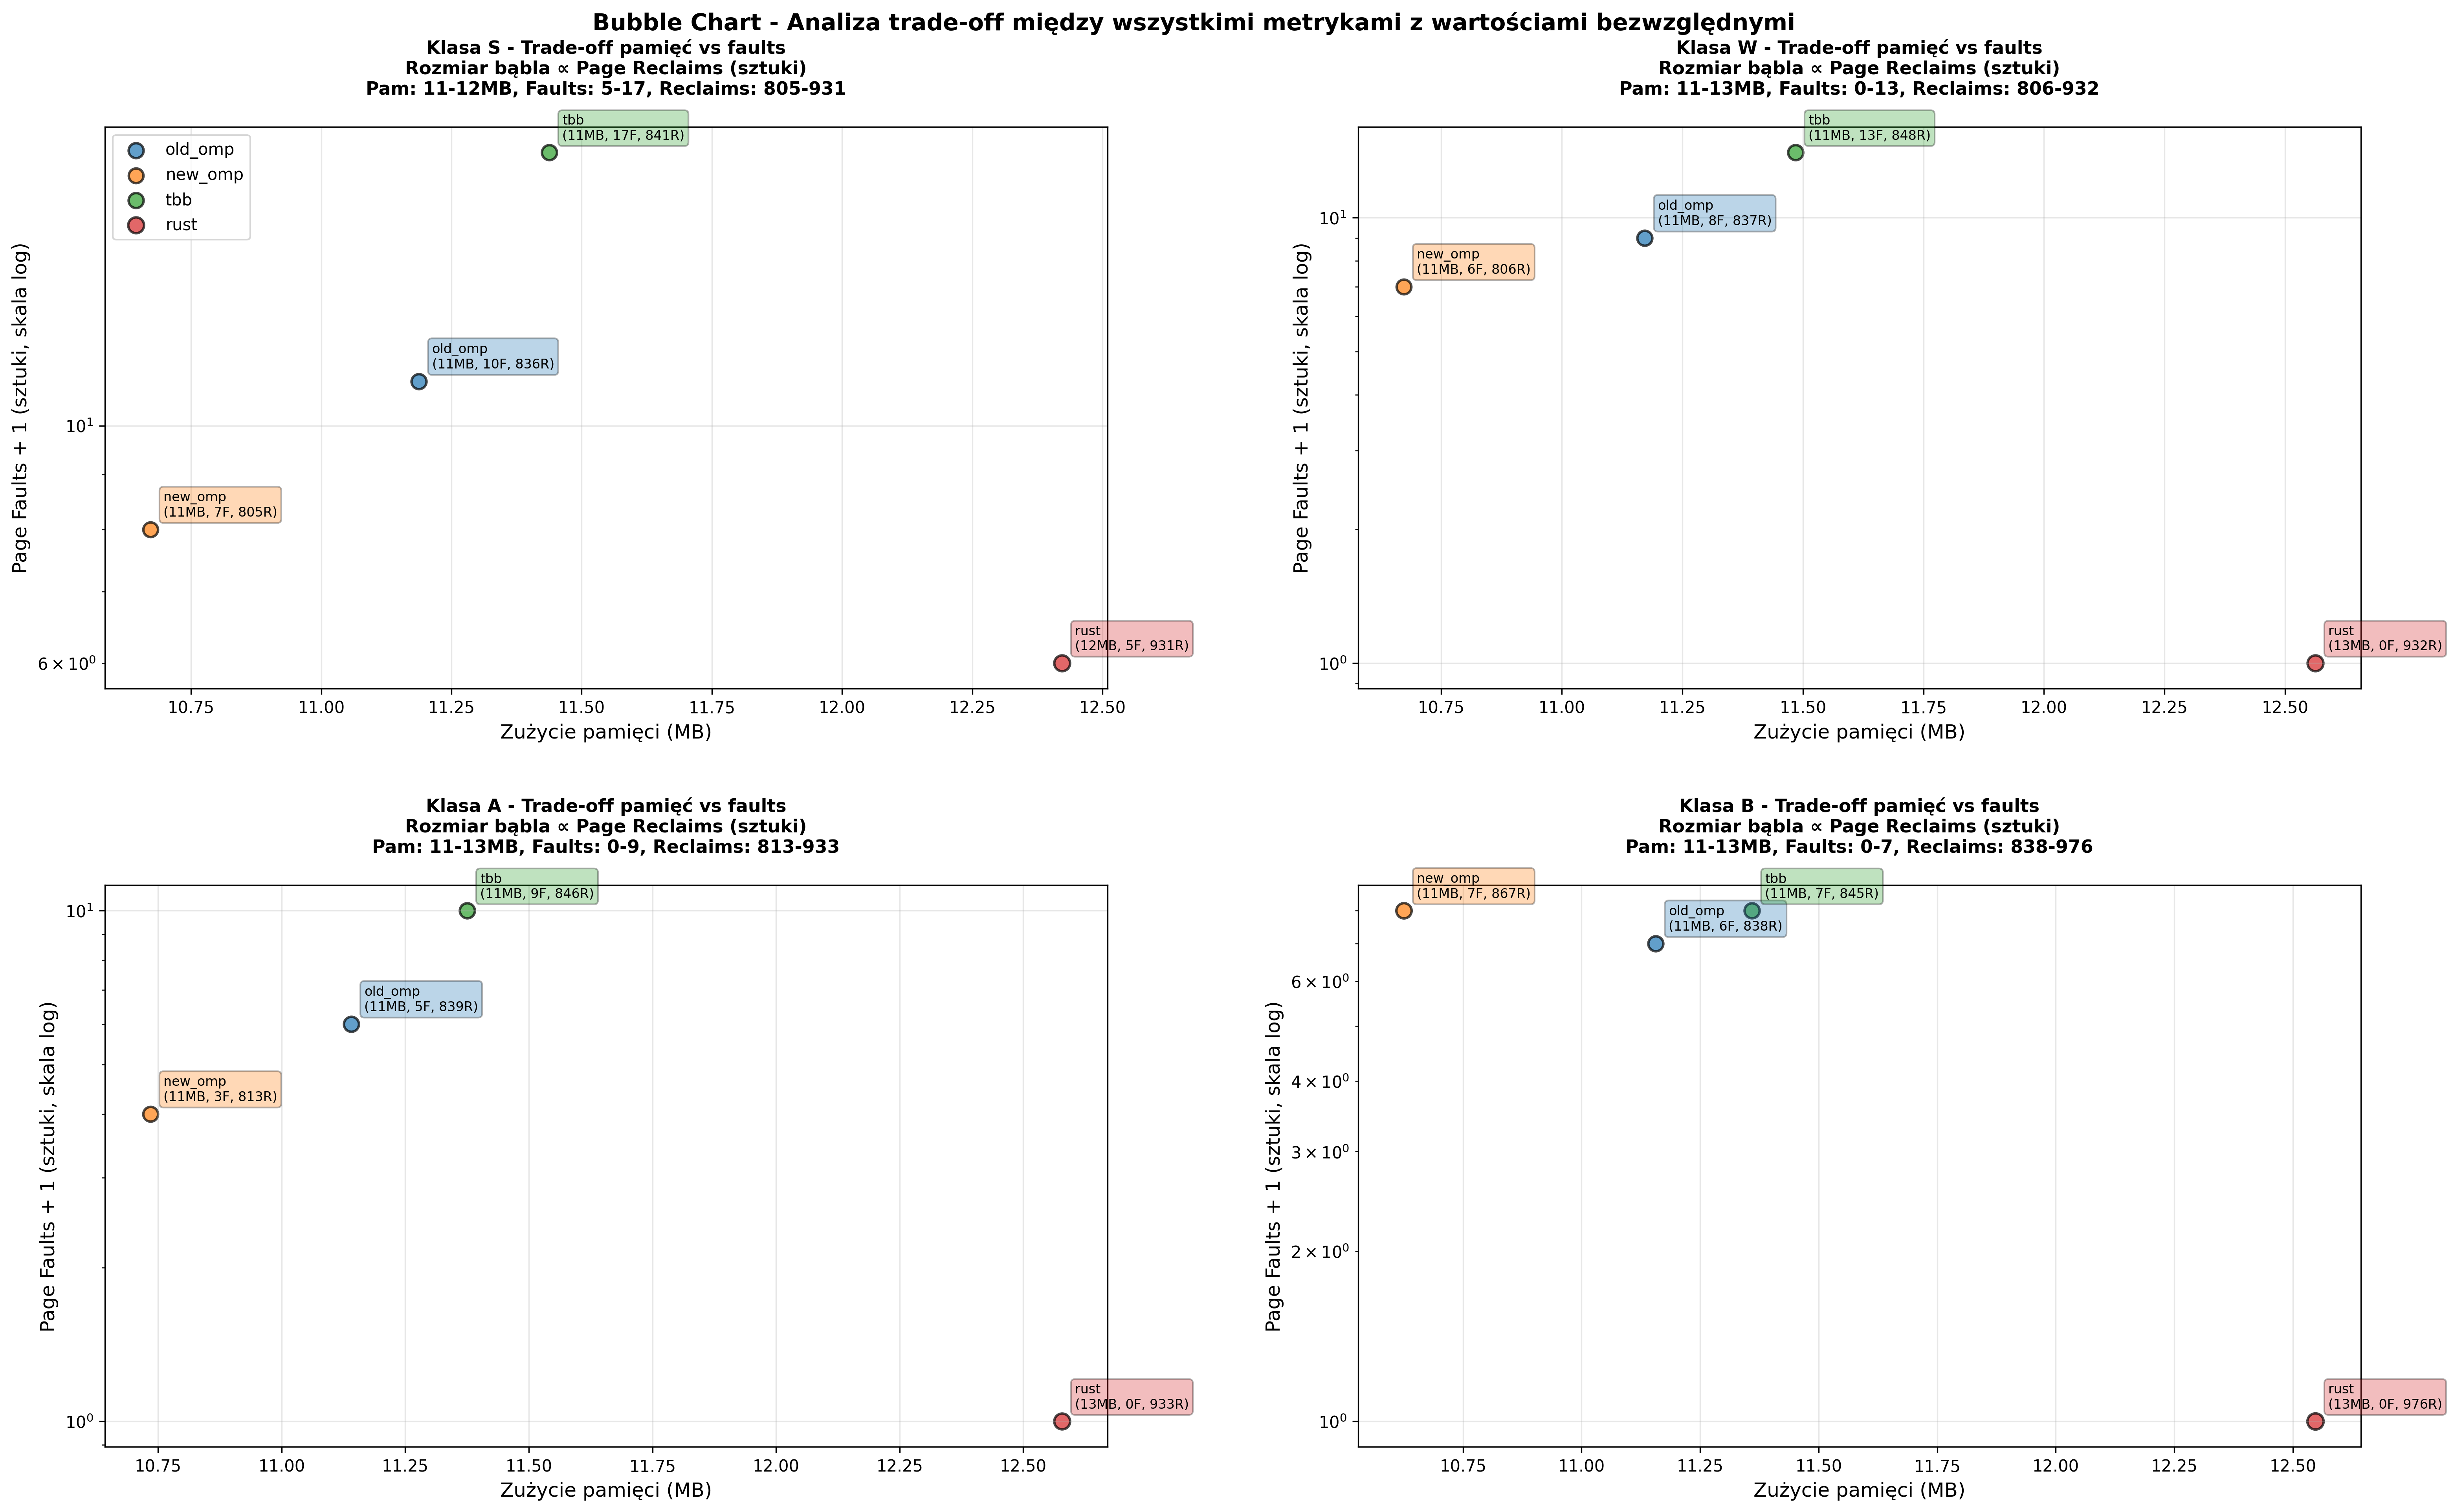
\includegraphics[width=\textwidth]{analiza/images/parallel/ep/chart_06_bubble_chart.png}
    \caption{Kompromisy \eng{trade-off} pomiędzy zużyciem pamięci a błędami stron pamięci, z uwzględnieniem liczby odzyskanych stron jako trzeciej zmiennej reprezentowanej przez rozmiar bąbla}
    \label{ep_kompromisy_pamiec_bledy}
\end{figure}
Rysunek \ref{ep_kompromisy_pamiec_bledy} przedstawia kompromisy\eng{trade-offs} między zużyciem pamięci a błędami stron, z liczbą odzyskanych stron jako trzecim wymiarem (rozmiar bąbla). Oś Y jest przedstawiona w skali logarytmicznej ze względu na zróżnicowaną skalę błędów stron.

Najbardziej zrównoważone profile (niska pamięć i niski poziom błędów) osiągają new\_omp i częściowo old\_omp. tbb prezentuje najwyższy poziom błędów stron, natomiast rust, mimo wysokiego zużycia pamięci i największej liczby zwolnionych stron, całkowicie eliminuje błędy stron, co czyni go atrakcyjnym w kontekstach wymagających wysokiej niezawodności pamięciowej.

\subsection{Wyniki profilowania wydajności - platforma x86\_64}